% L9b student companion deck: American exercise on a CRR lattice.
%
% The frame order mirrors the lecture notebook so students can take notes while
% the instructor works through the notebook. The disclaimer is intentionally
% slide 2, by instructor preference.
%
% Notation follows the lecture notebook: the risk-neutral up
% probability is q, matching L3b, which reserves p for the real-world up
% probability; the continuously compounded rate is g_y, matching L2a and L9a;
% lattice nodes are indexed (t,k) with t the level and k the number of up moves,
% matching L3b and L4a. Payoff functions h_c/h_p are L8b/L9a's; H is the generic
% payoff of whichever contract is being priced. There is no opening
% concept-review section in the notebook, so there is no \transitionframe.
\documentclass[aspectratio=169,11pt]{beamer}
\usepackage{vnslides}

\newcommand{\R}{\mathbb{R}}
\newcommand{\gy}{g_y}
\newcommand{\dt}{\Delta t}
\newcommand{\AM}{\mathrm{AM}}
\newcommand{\EU}{\mathrm{EU}}

\title{\texorpdfstring{{\vnheavy L9b}}{L9b}: American Options, CRR Pricing, and the Value of Early Exercise}
\subtitle{CHEME 5660 Cornell University}
\author{Copyright Jeffrey Varner 2026. All Rights Reserved}

\begin{document}

\vntitlepage

\begin{frame}{Disclaimer and Risks}
  \vspace{0.6em}
  \textbf{\ink{Training only.}} This content is for training and informational
  purposes only. The teaching team does not make, give, or endorse any offer or
  solicitation to buy or sell securities or derivative products, or provide
  investment or trading advice or strategy.

  \vspace{1.1em}
  \textbf{\ink{Risk.}} Trading involves risk and is generally not recommended for
  those with limited resources, experience, or a low risk tolerance. Past
  performance does not guarantee future success.

  \vspace{1.1em}
  \textbf{\ink{Responsibility.}} You are responsible for your investment decisions
  based on your financial circumstances, objectives, risk tolerance, and
  liquidity needs.
\end{frame}

\begin{frame}{Objectives for Today}
  L9a priced contracts exercisable only at expiration. Today the holder gets a
  \hilite{choice of when to exercise}. We keep the same terminal payoffs, price
  both exercise styles on one lattice, and measure what that extra right is
  worth.

  \vspace{0.5em}
  {\large\textbf{\ink{Today's concepts}}}
  \begin{itemize}\setlength{\itemsep}{0.4em}
    \item \hilite{Contrast European and American exercise}: explain why identical
      terminal payoffs can carry different premiums when one holder may exercise
      early.
    \item \hilite{Price both styles on one CRR lattice}: apply the European and
      American backward-induction rules under identical inputs and verify that
      the American value is never smaller.
    \item \hilite{Explain the premium difference}: separate intrinsic value,
      extrinsic value, and the early-exercise premium, and identify when the
      American premium is strictly higher.
  \end{itemize}
\end{frame}

\begin{frame}{Lectures and Examples}
  \textbf{\ink{Lecture:}} the American exercise set, the CRR lattice, the two
  backward-induction rules, the three value differences, and the conditions
  under which American exercise is actually worth something.

  \vspace{0.8em}
  \textbf{\ink{Example 1:}} the two-step textbook put. Price both styles on one
  lattice and inspect the node where exercise beats continuation.

  \vspace{0.55em}
  \textbf{\ink{Example 2:}} an AMD option chain. Price the whole chain with CRR
  under both rules and compare with quoted bid-ask intervals.

  \vspace{0.55em}
  \textbf{\ink{Example 3:}} an NVDA call. Split the premium into intrinsic and
  extrinsic value across strike and time to expiration.
\end{frame}

\begin{frame}{Same Terminal Payoff, Different Exercise Set}
  For strike $K>0$ and underlying price $S\geq0$, with $x^{+}:=\max(x,0)$, the
  immediate-exercise values are:
  \[
    h_c(S)=(S-K)^{+},\qquad h_p(S)=(K-S)^{+}.
  \]
  \begin{itemize}\setlength{\itemsep}{0.4em}
    \item \hilite{European}: receives this payoff only at expiration $T$.
    \item \hilite{American}: may choose any exercise time $\tau\leq T$, which
      includes the strategy of never exercising early.
  \end{itemize}
  The American strategy set \hilite{contains} the European one, so under
  identical model inputs:
  \[
    \boxed{V_0^{\AM}\geq V_0^{\EU}.}
  \]
  The inequality need not be strict.
\end{frame}

\begin{frame}{Build the Cox--Ross--Rubinstein Lattice}
  Split maturity $T$ into $N$ steps of length $\dt=T/N$. With continuously
  compounded risk-free rate $\gy$ and annualized volatility $\sigma>0$, CRR sets
  the move sizes and the pricing weight $q$:
  \[
    u=e^{\sigma\sqrt{\dt}},\quad d=e^{-\sigma\sqrt{\dt}},
    \qquad
    \boxed{q=\frac{e^{\gy\dt}-d}{u-d}.}
  \]
  \begin{itemize}\setlength{\itemsep}{0.25em}
    \item This is \hilite{L3b's one-step result} for a continuous rate: there
      $R_f=e^{\gy\dt}$ and $q=(R_f-d)/(u-d)$.
    \item $q$ is a \hilite{pricing weight}, not a forecast. L3b keeps $p$ for the
      real-world up probability; only $q$ appears today.
    \item No arbitrage requires $d<e^{\gy\dt}<u$, equivalently $0<q<1$. If that
      fails, \hilite{refine the step}, never clip $q$.
    \item With a continuous dividend yield $\delta$, replace $e^{\gy\dt}$ in the
      numerator by $e^{(\gy-\delta)\dt}$.
  \end{itemize}
\end{frame}

\begin{frame}{One Lattice, Two Backward-Induction Rules}
  Index a node by its level $t\in\{0,\dots,N\}$ and its number of up moves
  $k\in\{0,\dots,t\}$, so $S_{t,k}=S_0u^kd^{t-k}$, as in L3b and L4a. At
  expiration both styles agree, $V_{N,k}=h(S_{N,k})$, where $h$ is whichever of
  $h_c$, $h_p$ applies. For $t<N$ the discounted continuation value is:
  \[
    C_{t,k}=e^{-\gy\dt}\bigl[\,\underbrace{qV_{t+1,k+1}+(1-q)V_{t+1,k}}_{\text{pricing expectation}}\,\bigr].
  \]
  The exercise convention changes \hilite{exactly one line}:
  \[
    \boxed{V^{\EU}_{t,k}=C^{\EU}_{t,k}}
    \qquad
    \boxed{V^{\AM}_{t,k}=\max\bigl\{h(S_{t,k}),\,C^{\AM}_{t,k}\bigr\}.}
  \]
  Exercise where $h>C$, wait where $C>h$. Equality is indifference: the premium
  does not depend on the tie-break, the reported decision does.
\end{frame}

\begin{frame}{A Two-Step Put Makes the Difference Visible}
  Take $S_0=50$, $K=52$, two one-year steps, $u=1.2$, $d=0.8$, and $\gy=5\%$, so
  $q\approx0.6282$. Since $ud=0.96\neq1$ this is a \hilite{generic} binomial
  tree, not a CRR calibration; the two recursions are unchanged either way.

  \vspace{0.4em}
  At the one-year down node $S=40$, exercising pays $12$ while waiting is worth:
  \[
    e^{-0.05}\bigl[0.6282(4)+0.3718(20)\bigr]\approx9.46.
  \]
  The American holder \hilite{exercises}; the European holder must wait. Rolling
  both trees to the root:
  \[
    \boxed{V_0^{\EU}\approx4.19,\qquad V_0^{\AM}\approx5.09.}
  \]
  The early-exercise right is worth about $0.90$ USD/share here.
  \slidenote{Example 1:}{\dimmed{CHEME-5660-L9b-Example-Hull-American-Put-Fall-2026.ipynb}}
\end{frame}

\begin{frame}{One Node Carries the Whole Difference}
  \vspace{-0.9em}
  \begin{center}
    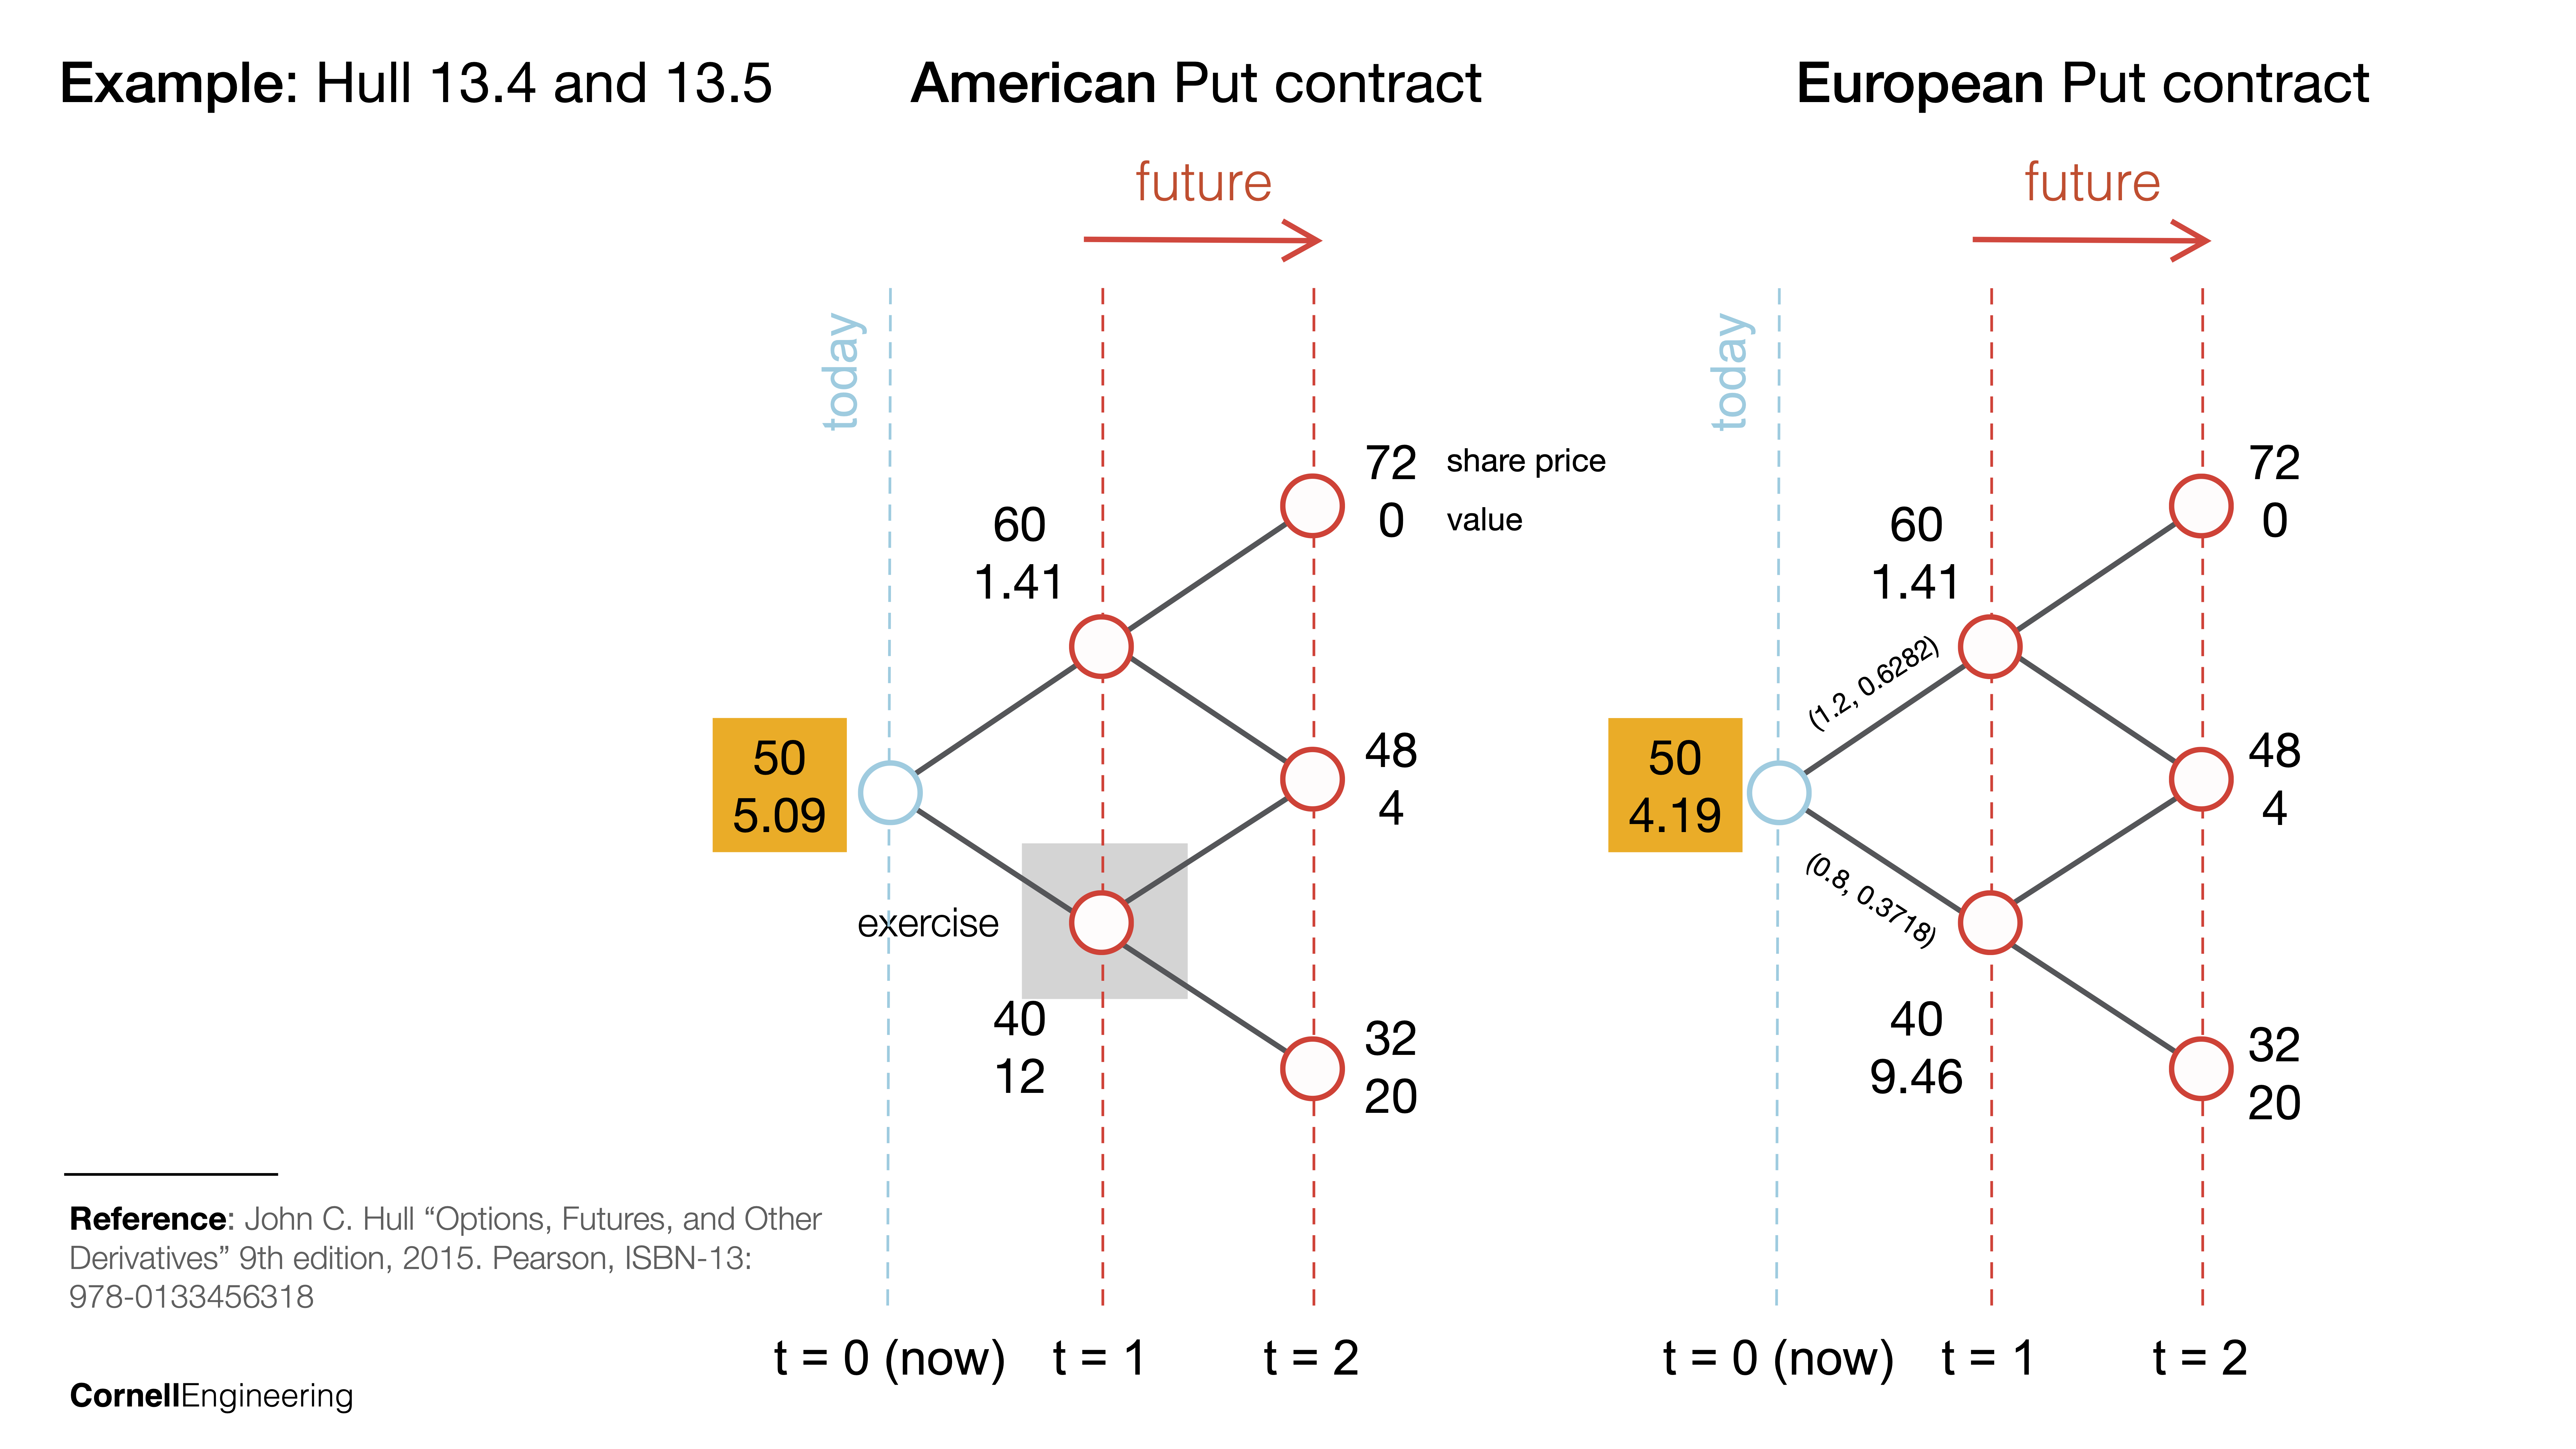
\includegraphics[width=0.84\textwidth,keepaspectratio]{../figs/Fig-HullExample-American-v-European-Schematic.png}
  \end{center}
  \vspace{-1.1em}
  Only the down node differs: American $12$, European $9.46$.
\end{frame}

\begin{frame}{Three Value Differences Answer Three Questions}
  Let $V$ be the optimally managed value, $h$ intrinsic value, and $C$
  continuation value. At an interior node, that is for $t<N$:
  \[
    \underbrace{X_{t,k}=V_{t,k}-h(S_{t,k})}_{\text{extrinsic value}}
    =\bigl(C_{t,k}-h(S_{t,k})\bigr)^{+}\geq0,
  \]
  because $\max\{h,C\}-h=\max\{0,C-h\}$. Continuation is undefined at
  expiration, where $V_{N,k}=h(S_{N,k})$ gives $X_{N,k}=0$ directly. Across
  styles:
  \[
    \underbrace{A=V^{\AM}-V^{\EU}}_{\text{early-exercise premium}}\geq0.
  \]
  \begin{itemize}\setlength{\itemsep}{0.2em}
    \item $C$: what is waiting worth?
    \item $X$: how far does the managed contract exceed immediate exercise?
    \item $A$: what does American flexibility add over the same European contract?
  \end{itemize}
\end{frame}

\begin{frame}{When Is the American Premium Strictly Higher?}
  \begin{itemize}\setlength{\itemsep}{0.4em}
    \item \hilite{Non-dividend calls, $\gy\geq0$}: early exercise is never
      strictly better, so $V_c^{\AM}=V_c^{\EU}$. Paying $K$ early and discarding
      optionality cannot help. For $\gy>0$ waiting is strictly better; at
      $\gy=0$ the holder can be indifferent.
    \item \hilite{Puts}: early exercise can be optimal. Receiving $K$ sooner has
      financing value, but that has to \hilite{exceed the optionality given up},
      which is why the put must also be sufficiently in the money.
    \item \hilite{Dividend-paying calls}: exercising before an ex-dividend date
      can pay when the dividend beats retaining the option and deferring $K$.
    \item \hilite{Negative rates, discrete dividends, funding spreads,
      constraints}: each needs its own model before any exercise rule follows.
  \end{itemize}
  \vspace{0.2em}
  American style guarantees only the \hilite{weak} inequality.
  \slidenote{Examples 2 and 3:}{\dimmed{AMD chain premiums; NVDA intrinsic and extrinsic value}}
\end{frame}

% ==== optional advanced material =============================
\begin{frame}{Optional Advanced Material}
  \vspace{0.4em}
  {\normalsize\textbf{\ink{Advanced:}} \dimmed{advanced/crr\_factors/}\par
  \dimmed{CHEME-5660-L9b-Advanced-CRR-Factors-Fall-2026.ipynb}}

  \vspace{0.7em}
  Optional, not a prerequisite for L10a. Today's lecture \hilite{quotes}
  $u=e^{\sigma\sqrt{\dt}}$ and $d=e^{-\sigma\sqrt{\dt}}$; the notebook derives
  them. It writes the one-step log return as a two-point variable and matches its
  variance to the diffusion variance $\sigma^{2}\dt$, and it is explicit about
  the price: $ud=1$ is a \hilite{normalization the modeler chooses}, not
  something the diffusion forces, the equal weights used to size the jump are
  \hilite{not} the pricing probability $q$, and the variance match holds only to
  leading order, discarding a term of order $\dt^{2}$. It closes with the domain
  $\lvert\gy\rvert\sqrt{\dt}<\sigma$ that keeps $0<q<1$.
  \slidenote{Notebook:}{\href{https://github.com/varnerlab/CHEME-5660-CourseRepository-Fall-2026/tree/main/lectures/week-9/L9b/advanced}{lectures/week-9/L9b/advanced}, also linked from the lecture notebook.}
\end{frame}

\begin{frame}{Summary}
  Today we took L9a's European price as a benchmark, added the American exercise
  decision on the same lattice, and measured what that extra right is worth.

  {\large\textbf{\ink{Key takeaways}}}
  \begin{itemize}\setlength{\itemsep}{0.15em}
    \item \hilite{American style expands the exercise set}: the American holder
      can always choose to wait until expiration, so the American premium is
      never smaller than the European premium under identical inputs.
    \item \hilite{Backward induction creates the difference}: the European
      recursion always continues, the American recursion takes the larger of
      intrinsic and continuation value, and that one line is the whole
      distinction.
    \item \hilite{Higher is not automatic}: on the AMD chain the American and
      European call premiums agree exactly, while the puts carry a
      positive early-exercise premium that reaches about $2.30$ USD/share at the
      deepest in-the-money strike.
  \end{itemize}
  Next, L10a asks how a premium responds locally to spot, volatility, time, and
  interest rates through the Greeks.
\end{frame}

\end{document}
